\documentclass{beamer}

% -------------------------------------------------------------------
% 1. PACKAGES
% -------------------------------------------------------------------
\usepackage{tikz}
\usetikzlibrary{shapes, arrows.meta, positioning, shadows, trees, fit, backgrounds, automata, quotes, intersections}
\usepackage{graphicx}
\usepackage{xcolor}
\usepackage{booktabs}
\usepackage{adjustbox}
\usepackage{ragged2e} % For justified text in columns

% -------------------------------------------------------------------
% 2. THEME & COLORS
% -------------------------------------------------------------------
\usetheme{Madrid}
\setbeamertemplate{navigation symbols}{}

\definecolor{DeepOrange}{RGB}{230,81,0}
\definecolor{LightOrange}{RGB}{255,167,38}
\definecolor{PaleOrange}{RGB}{255,243,224}

\usecolortheme[named=DeepOrange]{structure}
\setbeamercolor{palette primary}{bg=DeepOrange, fg=white}
\setbeamercolor{palette secondary}{bg=DeepOrange!80, fg=white}
\setbeamercolor{block title}{bg=DeepOrange, fg=white}
\setbeamercolor{block body}{bg=DeepOrange!10, fg=black}

% -------------------------------------------------------------------
% 3. CUSTOM BACKGROUND DECORATION
% -------------------------------------------------------------------
\setbeamertemplate{background canvas}{
  \begin{tikzpicture}[remember picture, overlay]

    % Top-right soft curve
    \fill[LightOrange!20]
      (current page.north east)
      -- +(-5cm,0)
      .. controls +(-1cm,-2cm) and +(0,-2cm) ..
      +(0,-4.5cm)
      -- cycle;

    % Sharp corner accent
    \fill[DeepOrange]
      (current page.north east)
      -- +(-0.8cm,0)
      -- +(0,-0.8cm)
      -- cycle;

    % Bottom-left sidebar
    \fill[DeepOrange!10]
      (current page.south west) rectangle +(0.8cm,5cm);

    % Footer block
    \fill[DeepOrange]
      (current page.south west) rectangle +(0.8cm,0.4cm);

    % Floating shapes
    \draw[DeepOrange!10, line width=2pt] (10,3) circle (2.5cm);
    \fill[LightOrange!30] (1,8) circle (0.4cm);

    % Line accents
    \draw[DeepOrange!40, thick] (11,0.5) -- (12.5,0.5);
    \draw[DeepOrange!40, thick] (11.5,0.3) -- (12.5,0.3);

  \end{tikzpicture}
}

% -------------------------------------------------------------------
% 4. METADATA
% -------------------------------------------------------------------
\title{Large Language Models}
\subtitle{Comprehensive Overview and Future Directions}
\author{Academic Presentation Designer}
\date{\today}

% -------------------------------------------------------------------
% 5. CUSTOM COMMANDS FOR GLOBAL FOOTNOTES AND BIBLIOGRAPHY
% -------------------------------------------------------------------
\newcounter{mybibcounter}
\newcommand{\mybiblist}{} % Stores the full bibliography items

% Command to add a reference and get its globally consistent number
\newcommand{\refer}[2]{% #1 = short citation (e.g., Brown et al. 2020), #2 = full bibliography entry
  \ifcsundef{refnum#1}{%
    % First time this reference is cited, assign a new number
    \stepcounter{mybibcounter}%
    \expandafter\xdef\csname refnum#1\endcsname{\arabic{mybibcounter}}%
    % Add to the bibliography list
    \xappto\mybiblist{\bibitem[\arabic{mybibcounter}]{#1}#2}%
  }{}%
  % Output the footnote with the assigned global number
  \footnote{\scriptsize [\csname refnum#1\endcsname] #1}%
}

\begin{document}

% --- TITLE SLIDE ---
\begin{frame}
  \titlepage
\end{frame}

% --- OVERVIEW SLIDE ---
\begin{frame}{Overview}
  \tableofcontents
\end{frame}

% --- CONTENT SLIDES ---

\section{Introduction to Large Language Models (LLMs)}

% Slide 1.1: Deep Dive - What are LLMs?
\begin{frame}{What are Large Language Models (LLMs)?}
  \begin{columns}
    \begin{column}{0.5\textwidth}
      \begin{itemize}
        \item LLMs are advanced artificial intelligence models designed to understand and generate human-like text.
        \item They are built upon the \textbf{Transformer architecture}\addreference{Vaswani et al. 2017. Attention Is All You Need}, enabling efficient processing of sequential data.
        \item Trained on vast amounts of text data, LLMs learn complex patterns, grammar, and factual information.
        \item Capabilities include text completion, summarization, translation, and question and answer (Q\&A).
      \end{itemize}
    \end{column}
    \begin{column}{0.5\textwidth}
      \begin{adjustbox}{max width=\textwidth, max totalheight=0.6\textheight, center}
        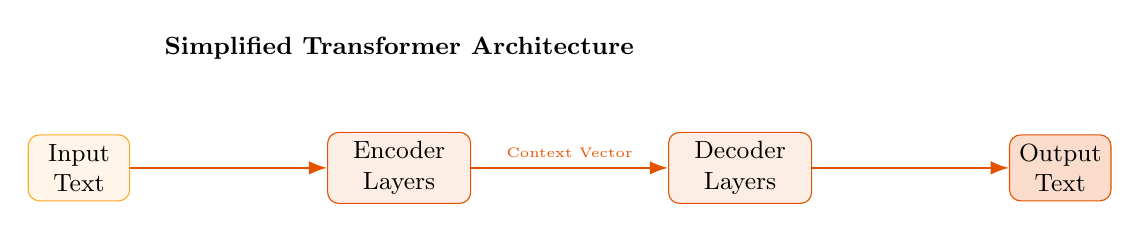
\begin{tikzpicture}[
          node distance=1.5cm,
          block/.style={rectangle, draw=DeepOrange, fill=DeepOrange!10, text width=4.5em, text centered, rounded corners, minimum height=2em, font=\small},
          arrow/.style={-Latex, thick, DeepOrange},
          input/.style={rectangle, draw=LightOrange, fill=LightOrange!10, text width=3em, text centered, rounded corners, minimum height=2em, font=\small},
          output/.style={rectangle, draw=DeepOrange, fill=DeepOrange!20, text width=3em, text centered, rounded corners, minimum height=2em, font=\small}
        ]
          \node (input) [input] {Input Text};
          \node (encoder) [block, right=of input, xshift=1cm] {Encoder Layers};
          \node (decoder) [block, right=of encoder, xshift=1cm] {Decoder Layers};
          \node (output) [output, right=of decoder, xshift=1cm] {Output Text};

          \draw [arrow] (input) -- (encoder);
          \draw [arrow] (encoder) -- node[above, font=\tiny] {Context Vector} (decoder);
          \draw [arrow] (decoder) -- (output);

          \node[above=0.8cm of encoder.north, text width=6cm, align=center, font=\small\bfseries] {Simplified Transformer Architecture};
        \end{tikzpicture}
      \end{adjustbox}
    \end{column}
  \end{columns}
\end{frame}

% Slide 1.2: List - Key Capabilities & Evolution
\begin{frame}{Key Capabilities and Evolution}
  \begin{columns}
    \begin{column}{0.48\textwidth}
      \textbf{Core Capabilities}
      \begin{itemize}
        \item \textbf{Content Generation:} Crafting human-like articles, stories, and code.
        \item \textbf{Information Retrieval:} Answering complex questions from vast knowledge bases.
        \item \textbf{Text Summarization:} Condensing long documents into concise summaries.
        \item \textbf{Translation \& Adaptation:} Bridging language barriers and stylistic changes.
      \end{itemize}
    \end{column}
    \begin{column}{0.48\textwidth}
      \textbf{Evolutionary Milestones}\addreference{Brown et al. 2020. Language Models are Few-Shot Learners}
      \begin{adjustbox}{max width=\textwidth, max totalheight=0.6\textheight, center}
        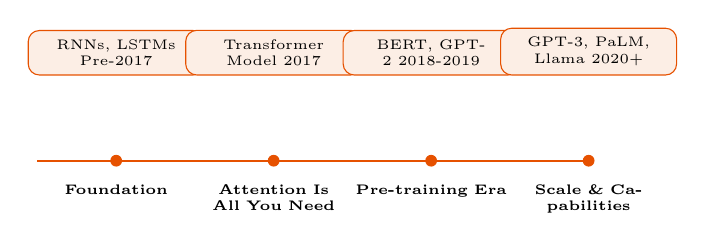
\begin{tikzpicture}[
          event/.style={rectangle, draw=DeepOrange, fill=DeepOrange!10, text width=2cm, text centered, rounded corners, minimum height=1.5em, font=\tiny},
          line/.style={DeepOrange, thick},
          point/.style={circle, fill=DeepOrange, inner sep=1.5pt},
          date/.style={below=0.1cm of #1, font=\tiny, text width=2cm, align=center}
        ]
          \coordinate (start) at (0,0);
          \coordinate (end) at (7,0);
          \draw[line] (start) -- (end);

          \node (p1) [point] at (1,0) {};
          \node (e1) [event, above=of p1] {RNNs, LSTMs Pre-2017};
          \node [date=p1] {\textbf{Foundation}};

          \node (p2) [point] at (3,0) {};
          \node (e2) [event, above=of p2] {Transformer Model 2017};
          \node [date=p2] {\textbf{Attention Is All You Need}};

          \node (p3) [point] at (5,0) {};
          \node (e3) [event, above=of p3] {BERT, GPT-2 2018-2019};
          \node [date=p3] {\textbf{Pre-training Era}};

          \node (p4) [point] at (7,0) {};
          \node (e4) [event, above=of p4] {GPT-3, PaLM, Llama 2020+};
          \node [date=p4] {\textbf{Scale \& Capabilities}};
        \end{tikzpicture}
      \end{adjustbox}
    \end{column}
  \end{columns}
\end{frame}

\section{Comparison of LLMs}

% Slide 2.1: Multi-Section - Diverse LLM Landscape
\begin{frame}{Diverse LLM Landscape}
  \begin{columns}
    \begin{column}{0.48\textwidth}
      \begin{enumerate}
        \item \textbf{Proprietary Models}
        \begin{itemize}
          \item Developed by private companies.
          \item Examples: OpenAI's GPT-4\addreference{OpenAI 2023. GPT-4 Technical Report}, Google's Gemini, Anthropic's Claude.
          \item Often offer cutting-edge performance, but with limited transparency.
        \end{itemize}
        \item \textbf{Open-Source Models}
        \begin{itemize}
          \item Publicly available models and weights.
          \item Examples: Meta's Llama 2, Falcon, Mistral.
          \item Enable broader research, customization, and deployment.
        \end{itemize}
      \end{enumerate}
    \end{column}
    \begin{column}{0.48\textwidth}
      \begin{adjustbox}{max width=\textwidth, max totalheight=0.6\textheight, center}
        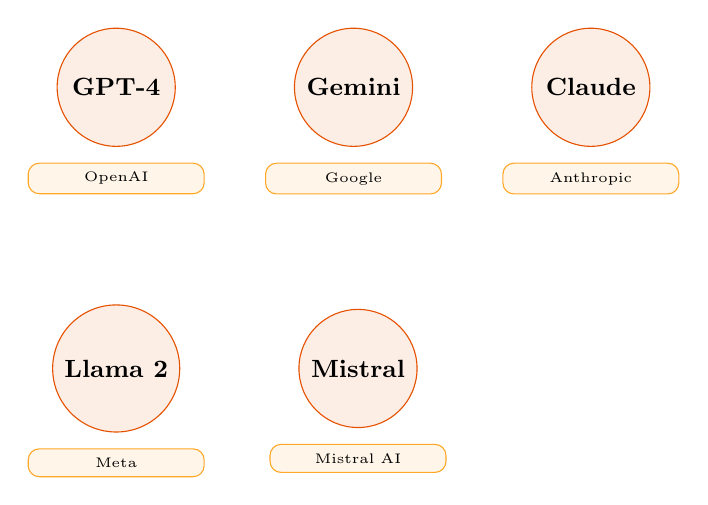
\begin{tikzpicture}[
          node distance=1.5cm,
          llm/.style={circle, draw=DeepOrange, fill=DeepOrange!10, minimum size=1.5cm, font=\small\bfseries, align=center},
          company/.style={rectangle, draw=LightOrange, fill=LightOrange!10, text width=2cm, text centered, rounded corners, minimum height=1em, font=\tiny},
          arrow/.style={-Latex, thick, DeepOrange!60}
        ]
          \node (gpt) [llm] {GPT-4};
          \node (openai) [company, below=0.2cm of gpt] {OpenAI};
          \node (gemini) [llm, right=1.5cm of gpt] {Gemini};
          \node (google) [company, below=0.2cm of gemini] {Google};
          \node (claude) [llm, right=1.5cm of gemini] {Claude};
          \node (anthropic) [company, below=0.2cm of claude] {Anthropic};
          \node (llama) [llm, below=2cm of gpt] {Llama 2};
          \node (meta) [company, below=0.2cm of llama] {Meta};
          \node (mistral) [llm, right=1.5cm of llama] {Mistral};
          \node (mistralai) [company, below=0.2cm of mistral] {Mistral AI};
        \end{tikzpicture}
      \end{adjustbox}
    \end{column}
  \end{columns}
\end{frame}

% Slide 2.2: Comparison - Architecture & Scale
\begin{frame}{Architecture and Scale}
  \begin{columns}
    \begin{column}{0.48\textwidth}
      \begin{itemize}
        \item \textbf{Model Size:} LLMs range from billions to trillions of parameters, impacting their complexity and capability.
        \item \textbf{Training Data:} Gigabytes to terabytes of text and code data for learning.
        \item \textbf{Architectural Variants:}
        \begin{itemize}
          \item \textit{Decoder-only:} GPT-series, Llama (generative).
          \item \textit{Encoder-decoder:} T5, BART (sequence-to-sequence tasks).
        \end{itemize}
      \end{itemize}
    \end{column}
    \begin{column}{0.48\textwidth}
      \begin{adjustbox}{max width=\textwidth, max totalheight=0.6\textheight, center}
        \begin{tabular}{l l l}
          \toprule
          \textbf{Feature} & \textbf{GPT-4} & \textbf{Gemini Ultra}\addreference{Gemini Team, Google DeepMind 2023. Gemini: A Family of Highly Capable Multimodal Models} \\
          \midrule
          \textbf{Developer} & OpenAI & Google DeepMind \\
          \textbf{Parameters} & \textgreater 170B (estimated) & Proprietary, very large \\
          \textbf{Modality} & Text, Image Input & Text, Image, Audio, Video \\
          \textbf{Key Strengths} & Advanced reasoning, long context & Multimodality, generalist \\
          \bottomrule
        \end{tabular}
      \end{adjustbox}
    \end{column}
  \end{columns}
\end{frame}

% Slide 2.3: Deep Dive - Performance Benchmarks
\begin{frame}{Performance Benchmarks}
  \begin{columns}
    \begin{column}{0.5\textwidth}
      \begin{itemize}
        \item Benchmarks like MMLU (Massive Multitask Language Understanding) and HELM (Holistic Evaluation of Language Models)\addreference{Liang et al. 2022. Holistic Evaluation of Language Models} assess diverse capabilities.
        \item LLMs are evaluated on reasoning, common sense, factual knowledge, and mathematical abilities.
        \item Performance continually improves, with larger and more refined models consistently pushing state-of-the-art.
      \end{itemize}
    \end{column}
    \begin{column}{0.5\textwidth}
      \begin{adjustbox}{max width=\textwidth, max totalheight=0.6\textheight, center}
        \begin{tikzpicture}[
          bar/.style={fill=DeepOrange!50, draw=DeepOrange, rectangle, minimum height=0.5cm},
          axis/.style={thick, gray, -latex},
          label/.style={font=\tiny, anchor=west}
        ]
          % Axes
          \draw[axis] (0,0) -- (5,0) node[below=0.1cm] {LLM};
          \draw[axis] (0,0) -- (0,4) node[left=0.1cm] {Score (\%)};

          % Bars (adjust height based on conceptual performance)
          \pgfmathsetmacro{\h1}{2.5}
          \pgfmathsetmacro{\h2}{3.2}
          \pgfmathsetmacro{\h3}{3.7}

          \node[bar, minimum width=0.8cm, anchor=south west, fill=LightOrange!50] at (0.5,0) [minimum height=\h1 cm] {};
          \node[bar, minimum width=0.8cm, anchor=south west, fill=DeepOrange!50] at (2.0,0) [minimum height=\h2 cm] {};
          \node[bar, minimum width=0.8cm, anchor=south west, fill=LightOrange!50] at (3.5,0) [minimum height=\h3 cm] {};

          \node[below=0.1cm of 0.5,0, font=\tiny] {GPT-3};
          \node[below=0.1cm of 2.0,0, font=\tiny] {Claude 2};
          \node[below=0.1cm of 3.5,0, font=\tiny] {GPT-4};

          \node[above=0.8cm of 3.5,3.7, text width=6cm, align=center, font=\small\bfseries] {Conceptual Performance on MMLU};
        \end{tikzpicture}
      \end{adjustbox}
    \end{column}
  \end{columns}
\end{frame}

% Slide 2.4: List - Key Features & Specializations
\begin{frame}{Key Features and Specializations}
  \begin{columns}
    \begin{column}{0.48\textwidth}
      \textbf{Distinguishing Features}
      \begin{itemize}
        \item \textbf{Multimodality:} Processing and generating various data types (text, image, audio).
        \item \textbf{Long Context Windows:} Handling and understanding much larger inputs or conversations.
        \item \textbf{Tool Use:} Ability to interact with external tools (Application Programming Interfaces (APIs), databases) for enhanced functionality.
        \item \textbf{Code Generation \& Debugging:} Assisting in software development workflows.
      \end{itemize}
    \end{column}
    \begin{column}{0.48\textwidth}
      \begin{adjustbox}{max width=\textwidth, max totalheight=0.6\textheight, center}
        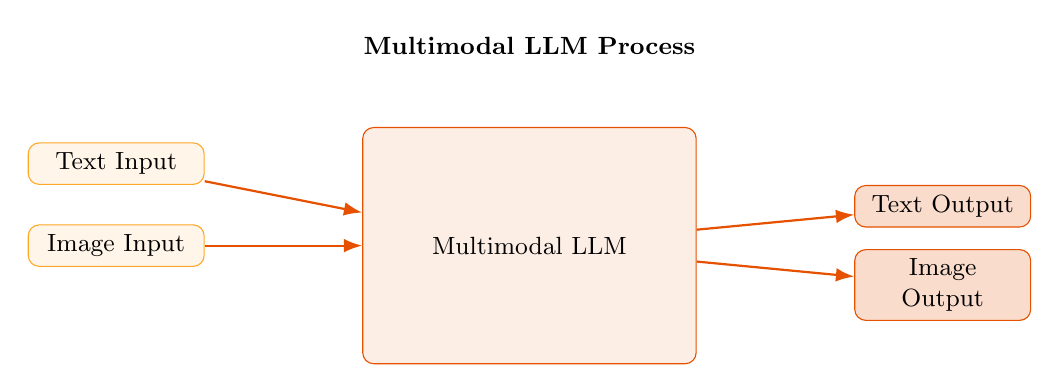
\begin{tikzpicture}[
          node distance=1cm,
          process/.style={rectangle, draw=DeepOrange, fill=DeepOrange!10, text width=3cm, text centered, rounded corners, minimum height=1.5em, font=\small},
          input/.style={rectangle, draw=LightOrange, fill=LightOrange!10, text width=2cm, text centered, rounded corners, minimum height=1.5em, font=\small},
          output/.style={rectangle, draw=DeepOrange, fill=DeepOrange!20, text width=2cm, text centered, rounded corners, minimum height=1.5em, font=\small},
          arrow/.style={-Latex, thick, DeepOrange}
        ]
          \node (text_in) [input] {Text Input};
          \node (image_in) [input, below=0.5cm of text_in] {Image Input};

          \node (llm) [process, right=2cm of text_in.east |- image_in.west, anchor=west, text width=4cm, minimum height=3cm] {Multimodal LLM};

          \node (text_out) [output, right=2cm of llm.east, yshift=0.5cm] {Text Output};
          \node (image_out) [output, right=2cm of llm.east, yshift=-0.5cm] {Image Output};

          \draw [arrow] (text_in) -- (llm);
          \draw [arrow] (image_in) -- (llm);
          \draw [arrow] (llm) -- (text_out);
          \draw [arrow] (llm) -- (image_out);

          \node[above=0.8cm of llm, text width=6cm, align=center, font=\small\bfseries] {Multimodal LLM Process};
        \end{tikzpicture}
      \end{adjustbox}
    \end{column}
  \end{columns}
\end{frame}

% Slide 2.5: Alertblock - Open-Source vs. Proprietary
\begin{frame}{Open-Source vs. Proprietary LLMs}
  \begin{columns}
    \begin{column}{0.48\textwidth}
      \begin{alertblock}{Key Considerations}
        \begin{itemize}
          \item \textbf{Accessibility:} Open-source models (e.g., Llama 2) are freely available, promoting broader use.
          \item \textbf{Customization:} Open weights allow fine-tuning for specific applications and data.
          \item \textbf{Performance vs. Control:} Proprietary models often lead in raw performance, while open-source offers greater control and transparency.
          \item \textbf{Community Contribution:} Open-source fosters rapid innovation and diverse applications from a global community.
        \end{itemize}
      \end{alertblock}
    \end{column}
    \begin{column}{0.48\textwidth}
      \begin{adjustbox}{max width=\textwidth, max totalheight=0.6\textheight, center}
        \begin{tikzpicture}[
          set/.style = {ellipse, opacity=0.8, fill=DeepOrange!30, minimum width=4cm, minimum height=3cm, draw=DeepOrange, line width=1pt},
          label/.style = {font=\bfseries\small, text width=2cm, align=center}
        ]
          \node (open) [set] {};
          \node (prop) [set, right=of open, xshift=-1.5cm] {};

          \node at (open.north) [label] {Open-Source};
          \node at (prop.north) [label] {Proprietary};

          \node at (open.center) [font=\small, align=center, text width=2.5cm] {Transparency \\ Flexibility \\ Community};
          \node at (prop.center) [font=\small, align=center, text width=2.5cm] {Peak Perf. \\ Support \\ Control};

          \node at (intersection of open and prop) [font=\small, align=center, text width=2cm] {Advancements \\ LLM Capabilities};
        \end{tikzpicture}
      \end{adjustbox}
    \end{column}
  \end{columns}
\end{frame}

\section{Humans \& LLMs}

% Slide 3.1: Deep Dive - Prompt Engineering
\begin{frame}{Prompt Engineering: Guiding LLMs}
  \begin{columns}
    \begin{column}{0.5\textwidth}
      \begin{itemize}
        \item Prompt engineering is the art of crafting effective inputs to elicit desired outputs from LLMs\addreference{Kiesewetter et al. 2023. Prompting for better AI: The value of instructing large language models}.
        \item \textbf{Key Techniques:}
        \begin{itemize}
          \item \textit{Few-shot learning:} Providing examples in the prompt.
          \item \textit{Chain-of-thought prompting:} Guiding the model through intermediate reasoning steps.
          \item \textit{Role-playing:} Instructing the LLM to adopt a persona.
        \end{itemize}
        \item Effective prompts significantly enhance performance and mitigate undesirable behaviors.
      \end{itemize}
    \end{column}
    \begin{column}{0.5\textwidth}
      \begin{adjustbox}{max width=\textwidth, max totalheight=0.6\textheight, center}
        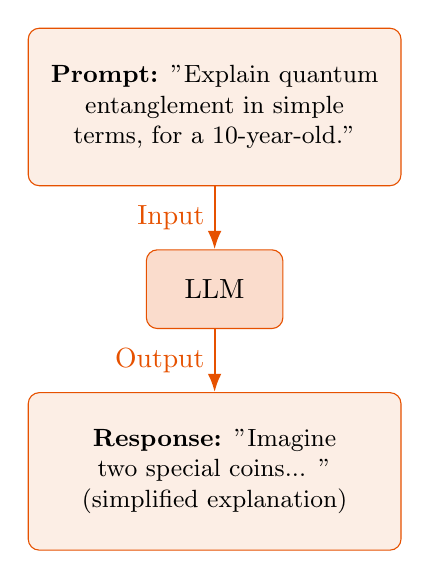
\begin{tikzpicture}[
          box/.style={rectangle, draw=DeepOrange, fill=DeepOrange!10, text width=4.5cm, minimum height=2cm, rounded corners, align=left, font=\small},
          arrow/.style={-Latex, thick, DeepOrange},
          label/.style={font=\tiny, text centered}
        ]
          \node (prompt) [box, align=center] {\textbf{Prompt:} "Explain quantum entanglement in simple terms, for a 10-year-old."};
          \node (llm) [rectangle, draw=DeepOrange, fill=DeepOrange!20, text width=1.5cm, text centered, minimum height=1cm, rounded corners, below=0.8cm of prompt] {LLM};
          \node (response) [box, below=0.8cm of llm, text width=4.5cm, align=center] {\textbf{Response:} "Imagine two special coins... " (simplified explanation)};

          \draw [arrow] (prompt) -- node[left] {Input} (llm);
          \draw [arrow] (llm) -- node[left] {Output} (response);
        \end{tikzpicture}
      \end{adjustbox}
    \end{column}
  \end{columns}
\end{frame}

% Slide 3.2: List - LLMs as Assistants
\begin{frame}{LLMs as Human Assistants}
  \begin{columns}
    \begin{column}{0.48\textwidth}
      \begin{itemize}
        \item LLMs are transforming various domains by acting as intelligent co-pilots and assistants.
        \item \textbf{Applications include:}
        \begin{itemize}
          \item \textit{Creative Writing:} Brainstorming ideas, generating drafts.
          \item \textit{Research Support:} Summarizing papers, extracting key information.
          \item \textit{Code Development:} Writing code snippets, debugging, documentation.
          \item \textit{Customer Service:} Automating responses, generating FAQs.
        \end{itemize}
        \item They augment human capabilities, allowing for increased efficiency and innovation.
      \end{itemize}
    \end{column}
    \begin{column}{0.48\textwidth}
      \begin{adjustbox}{max width=\textwidth, max totalheight=0.6\textheight, center}
        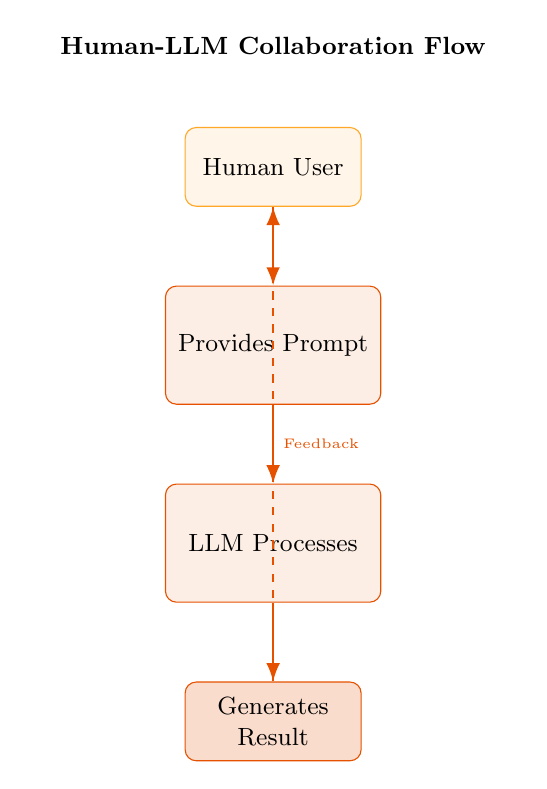
\begin{tikzpicture}[
          box/.style={rectangle, draw=DeepOrange, fill=DeepOrange!10, text width=2.5cm, minimum height=1.5cm, rounded corners, text centered, font=\small},
          arrow/.style={-Latex, thick, DeepOrange},
          input/.style={rectangle, draw=LightOrange, fill=LightOrange!10, text width=2cm, minimum height=1cm, rounded corners, text centered, font=\small},
          output/.style={rectangle, draw=DeepOrange, fill=DeepOrange!20, text width=2cm, minimum height=1cm, rounded corners, text centered, font=\small}
        ]
          \node (human) [input] {Human User};
          \node (prompt) [box, below=1cm of human] {Provides Prompt};
          \node (llm) [box, below=1cm of prompt] {LLM Processes};
          \node (result) [output, below=1cm of llm] {Generates Result};

          \draw [arrow] (human) -- (prompt);
          \draw [arrow] (prompt) -- (llm);
          \draw [arrow] (llm) -- (result);
          \draw [arrow, dashed] (result) -- node[right, font=\tiny] {Feedback} (human);

          \node[above=0.8cm of human, text width=6cm, align=center, font=\small\bfseries] {Human-LLM Collaboration Flow};
        \end{tikzpicture}
      \end{adjustbox}
    \end{column}
  \end{columns}
\end{frame}

% Slide 3.3: Exampleblock - Ethical Considerations
\begin{frame}{Ethical Considerations of LLMs}
  \begin{columns}
    \begin{column}{0.48\textwidth}
      \begin{exampleblock}{Ethical Challenges}
        \begin{itemize}
          \item \textbf{Bias and Fairness:} LLMs can perpetuate or amplify biases present in their training data.
          \item \textbf{Misinformation:} Potential for generating convincing but false or misleading content.
          \item \textbf{Accountability:} Attribution and responsibility for LLM-generated outputs remain complex.
          \item \textbf{Privacy:} Handling sensitive user data requires robust privacy safeguards.
        \end{itemize}
      \end{exampleblock}
    \end{column}
    \begin{column}{0.48\textwidth}
      \begin{adjustbox}{max width=\textwidth, max totalheight=0.6\textheight, center}
        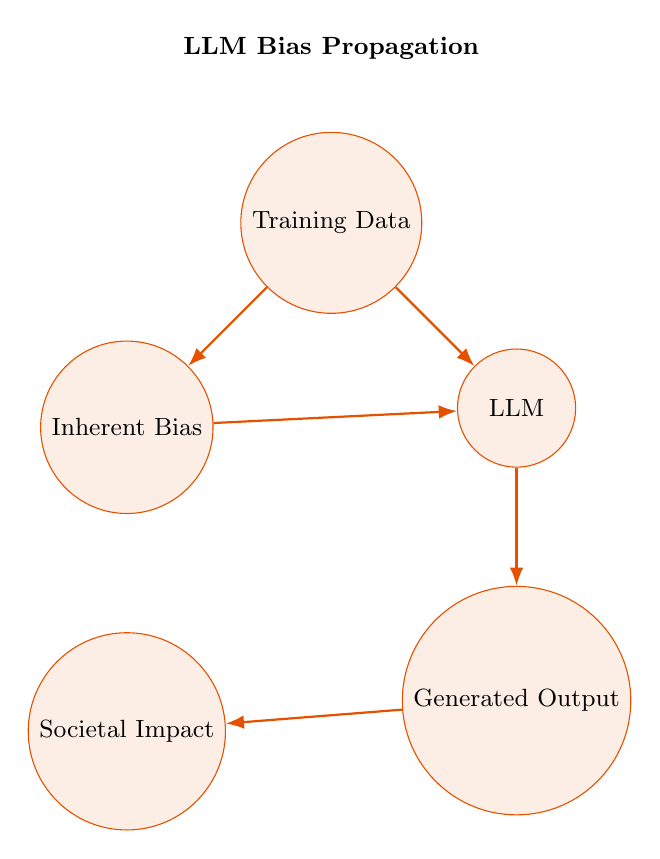
\begin{tikzpicture}[
          node distance=1.5cm,
          concept/.style={circle, draw=DeepOrange, fill=DeepOrange!10, minimum size=1.5cm, font=\small, text centered},
          link/.style={DeepOrange, thick, -Latex}
        ]
          \node (data) [concept] {Training Data};
          \node (bias) [concept, below left=1cm and 1cm of data] {Inherent Bias};
          \node (llm) [concept, below right=1cm and 1cm of data] {LLM};
          \node (output) [concept, below=1.5cm of llm] {Generated Output};
          \node (impact) [concept, below=1.5cm of bias] {Societal Impact};

          \draw[link] (data) -- (llm);
          \draw[link] (data) -- (bias);
          \draw[link] (bias) -- (llm);
          \draw[link] (llm) -- (output);
          \draw[link] (output) -- (impact);

          \node[above=0.8cm of data, text width=6cm, align=center, font=\small\bfseries] {LLM Bias Propagation};
        \end{tikzpicture}
      \end{adjustbox}
      \addreference{Bommasani et al. 2021. On the Opportunities and Risks of Foundation Models}
    \end{column}
  \end{columns}
\end{frame}

\section{Limitations of LLMs}

% Slide 4.1: Alertblock - Current Challenges
\begin{frame}{Current Limitations of LLMs}
  \begin{columns}
    \begin{column}{0.48\textwidth}
      \begin{alertblock}{Significant Challenges}
        \begin{itemize}
          \item \textbf{Factual Hallucinations:}\addreference{Ji et al. 2023. Survey of Hallucination in Large Language Models} Generating plausible but incorrect or fabricated information.
          \item \textbf{Training Data Bias:}\addreference{Blodgett et al. 2020. Language (Technology) is a Social Product} Reflecting and potentially amplifying biases present in their vast datasets.
          \item \textbf{Lack of True Understanding:}\addreference{Bender et al. 2021. On the Dangers of Stochastic Parrots} LLMs operate based on statistical patterns, not genuine comprehension or common sense.
          \item \textbf{Opacity (Black Box):} The decision-making process within complex models can be difficult to interpret.
        \end{itemize}
      \end{alertblock}
    \end{column}
    \begin{column}{0.48\textwidth}
      \begin{adjustbox}{max width=\textwidth, max totalheight=0.6\textheight, center}
        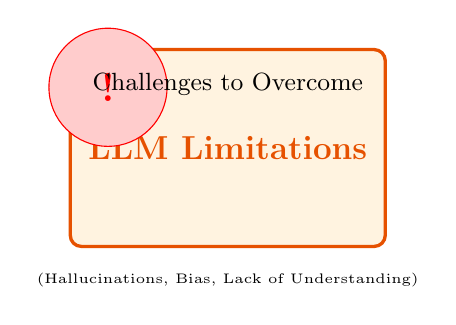
\begin{tikzpicture}[
          warning/.style={rectangle, draw=DeepOrange, fill=PaleOrange, very thick, rounded corners, minimum width=4cm, minimum height=2.5cm, align=center, font=\bfseries\large, text=DeepOrange},
          icon/.style={circle, draw=red, fill=red!20, minimum size=1.5cm, inner sep=0pt, font=\Huge\bfseries, text=red}
        ]
          \node (box) [warning] {LLM Limitations};
          \node [icon] at (box.north west) [xshift=0.5cm, yshift=-0.5cm] {\color{red}\Large !}; % Simple warning icon
          \node [below=0.2cm of box.north, font=\small] {Challenges to Overcome};
          \node [below=0.2cm of box.south, font=\tiny] {(Hallucinations, Bias, Lack of Understanding)};
        \end{tikzpicture}
      \end{adjustbox}
    \end{column}
  \end{columns}
\end{frame}

\section{Future Direction of LLMs}

% Slide 5.1: Deep Dive - Advancements & Research
\begin{frame}{Future Directions of LLMs}
  \begin{columns}
    \begin{column}{0.5\textwidth}
      \begin{itemize}
        \item \textbf{Multimodal Integration:}\addreference{Liu et al. 2024. Towards Universal Multimodal Large Language Models: A Survey} Seamless processing of text, images, audio, and video for richer interactions.
        \item \textbf{Enhanced Reasoning:} Developing models with better common sense and multi-step reasoning capabilities.
        \item \textbf{LLM-Powered Agents:}\addreference{Wang et al. 2023. A Survey on Large Language Model Based Agents} Creating autonomous agents that can plan, act, and reflect to achieve goals.
        \item \textbf{Ethical Alignment:} Focus on building more robust, steerable, and ethically aligned AI systems.
      \end{itemize}
    \end{column}
    \begin{column}{0.5\textwidth}
      \begin{adjustbox}{max width=\textwidth, max totalheight=0.6\textheight, center}
        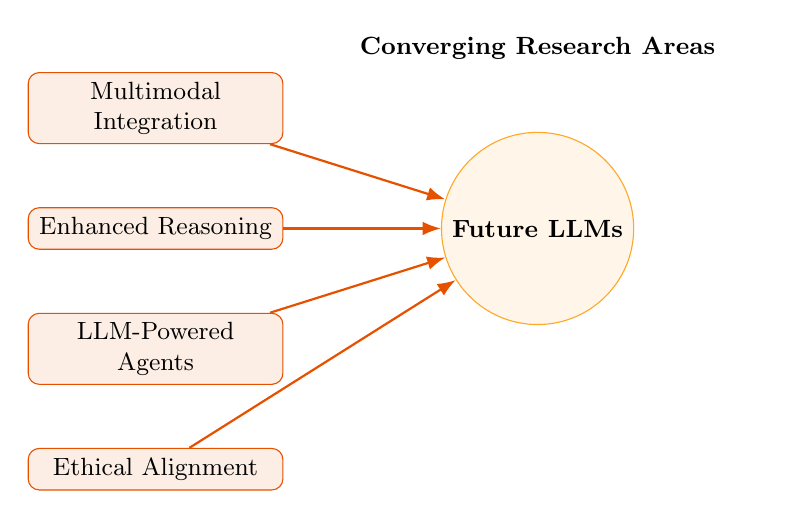
\begin{tikzpicture}[
          node distance=1.5cm,
          concept/.style={rectangle, draw=DeepOrange, fill=DeepOrange!10, text width=3cm, text centered, rounded corners, minimum height=1.5em, font=\small},
          arrow/.style={-Latex, thick, DeepOrange},
          start/.style={circle, draw=LightOrange, fill=LightOrange!10, minimum size=1cm, font=\small\bfseries}
        ]
          \node (multimodal) [concept] {Multimodal Integration};
          \node (reasoning) [concept, below=0.8cm of multimodal] {Enhanced Reasoning};
          \node (agents) [concept, below=0.8cm of reasoning] {LLM-Powered Agents};
          \node (ethics) [concept, below=0.8cm of agents] {Ethical Alignment};

          \node (center) [start, right=2cm of reasoning] {Future LLMs};

          \draw [arrow] (multimodal) -- (center);
          \draw [arrow] (reasoning) -- (center);
          \draw [arrow] (agents) -- (center);
          \draw [arrow] (ethics) -- (center);

          \node[above=0.8cm of center, text width=6cm, align=center, font=\small\bfseries] {Converging Research Areas};
        \end{tikzpicture}
      \end{adjustbox}
    \end{column}
  \end{columns}
\end{frame}

% --- REFERENCES SLIDE ---
\begin{frame}[allowframebreaks]{References}
  \footnotesize
  \RaggedRight % Ensure ragged right for better readability of long citations
  \begin{thebibliography}{99} % Use 99 for potentially many items
    \printtext{\mybiblist}
  \end{thebibliography}
\end{frame}

% --- CLOSING SLIDE ---
\begin{frame}
  \vfill
  \centering
  {\Huge \textbf{Thank You!}}
  \vfill
\end{frame}

\end{document}